% Document Class and Basic Packages
%-------------------------------------------------------------------------------
\documentclass[letterpaper,12pt]{article} % Define the document class and options
\usepackage{graphicx} % For including graphics
\usepackage[margin=1in]{geometry}
\usepackage{cite} % Handle citations
\usepackage[final]{hyperref} % Add hyperlinks
\usepackage{pgfplotstable, booktabs} % Enhance table handling
\usepackage{placeins} % Control float placement
\usepackage{tabularray} % Advanced tables
\usepackage{titlesec} % Customize section titles
\usepackage{fancyhdr} % Create custom page headers and footers
\usepackage{empheq} % Highlight equations
\usepackage{amssymb} % Extended math symbols
\usepackage{tcolorbox} % Colored boxes
\usepackage{enumitem} % Enhanced list environments
\usepackage{xcolor} % Define custom colors
%\usepackage{parskip} % Adjust paragraph spacing
\usepackage{siunitx} % Handling SI units
\usepackage{cancel} % Strikethrough text
\usepackage{listings} % Include code listings
\usepackage{tocloft}  % Table of contents formatting
\usepackage{mathtools}
\usepackage{pdfpages}
\usepackage{times}

% 1.5 spacing equivalent to word
\usepackage{setspace}
\linespread{1.25}


% Define Custom Colors
%-------------------------------------------------------------------------------
\definecolor{codegreen}{rgb}{0,0.6,0}
\definecolor{codegray}{rgb}{0.5,0.5,0.5}
\definecolor{codepurple}{rgb}{0.58,0,0.82}

% Define Code Listing Style
%-------------------------------------------------------------------------------
\lstdefinestyle{mystyle}{
    commentstyle=\color{codegreen},
    keywordstyle=\color{codepurple},
    numberstyle=\tiny\color{codegray},
    stringstyle=\color{codegreen},
    basicstyle=\ttfamily\small,
    breakatwhitespace=false,         
    breaklines=true,                 
    captionpos=b,                    
    keepspaces=true,                                                     
    showspaces=false,                
    showstringspaces=false,
    showtabs=false,                  
    tabsize=4
}

\DeclarePairedDelimiter\abs{\lvert}{\rvert}%
\DeclarePairedDelimiter\norm{\lVert}{\rVert}%

% Swap the definition of \abs* and \norm*, so that \abs
% and \norm resizes the size of the brackets, and the 
% starred version does not.
\makeatletter
\let\oldabs\abs
\def\abs{\@ifstar{\oldabs}{\oldabs*}}
%
\let\oldnorm\norm
\def\norm{\@ifstar{\oldnorm}{\oldnorm*}}
\makeatother

% Set Code Listing Style
\lstset{style=mystyle}

% Define Custom Commands and Settings
%-------------------------------------------------------------------------------
\newcommand*\widefbox[1]{\fbox{\hspace{0em}#1\hspace{0em}}} % Create a wide box
\newcommand{\tr}{\text{tr}} % Define a trace command for math mode

% Page Header and Footer Setup
%-------------------------------------------------------------------------------
\pagestyle{fancy} % Use the fancy page style
\fancyhf{} % Clear all header and footer fields
\fancyhead[L]{MEC E 301} % Left-aligned header
\fancyhead[C]{Lab 2: Digital Measurement Techniques} % Center header
\fancyhead[R]{Alex Diep} % Right-aligned header
\fancyfoot[C]{\thepage} % Centered page number in the footer

% Section and Subsection Formatting
%-------------------------------------------------------------------------------
\titleformat*{\section}{\Large\bfseries} % Customize section titles
\titleformat*{\subsection}{\large\bfseries} % Customize subsection titles
%\renewcommand{\thesection}{Question \arabic{section}} % Modify section numbering
%\renewcommand{\thesubsection}{(\alph{subsection})} % Modify subsection numbering

% Hyperlink Setup
%-------------------------------------------------------------------------------
\hypersetup{
	colorlinks=true, % Enable colored links
	linkcolor=blue, % Set link color
	citecolor=blue, % Set citation color
	filecolor=magenta, % Set file link color
	urlcolor=blue % Set URL link color
}

% Indentation Setup
%-------------------------------------------------------------------------------
%\newcommand{\forceindent}{{\setlength{\parindent}{2em}\indent}}

% Custom SI Unit Definitions
\DeclareSIUnit\LSB{LSB} % Least significant bit

% Custom Table of Contents Formatting
\renewcommand\cftsecdotsep{\cftdot} % Use dots for section 
\renewcommand{\cftsecleader}{\cftdotfill{\cftsubsecdotsep}} % Use subsection dots for section

\sisetup{group-digits=false} % changes the default (true)
% \titlespacing\section{0pt}{12pt plus 4pt minus 2pt}{0pt plus 2pt minus 2pt}
% \titlespacing\subsection{0pt}{12pt plus 4pt minus 2pt}{0pt plus 2pt minus 2pt}
% \titlespacing\subsubsection{0pt}{12pt plus 4pt minus 2pt}{0pt plus 2pt minus 2pt}
\titlespacing*{\section}{0pt}{0.1\baselineskip}{0.2\baselineskip}
\titlespacing*{\subsection}{0pt}{0.1\baselineskip}{0.2\baselineskip}
\titlespacing*{\subsubsection}{0pt}{0.1\baselineskip}{0.2\baselineskip}

% End of Preamble
%-------------------------------------------------------------------------------

%++++++++++++++++++++++++++++++++++++++++
\begin{document}

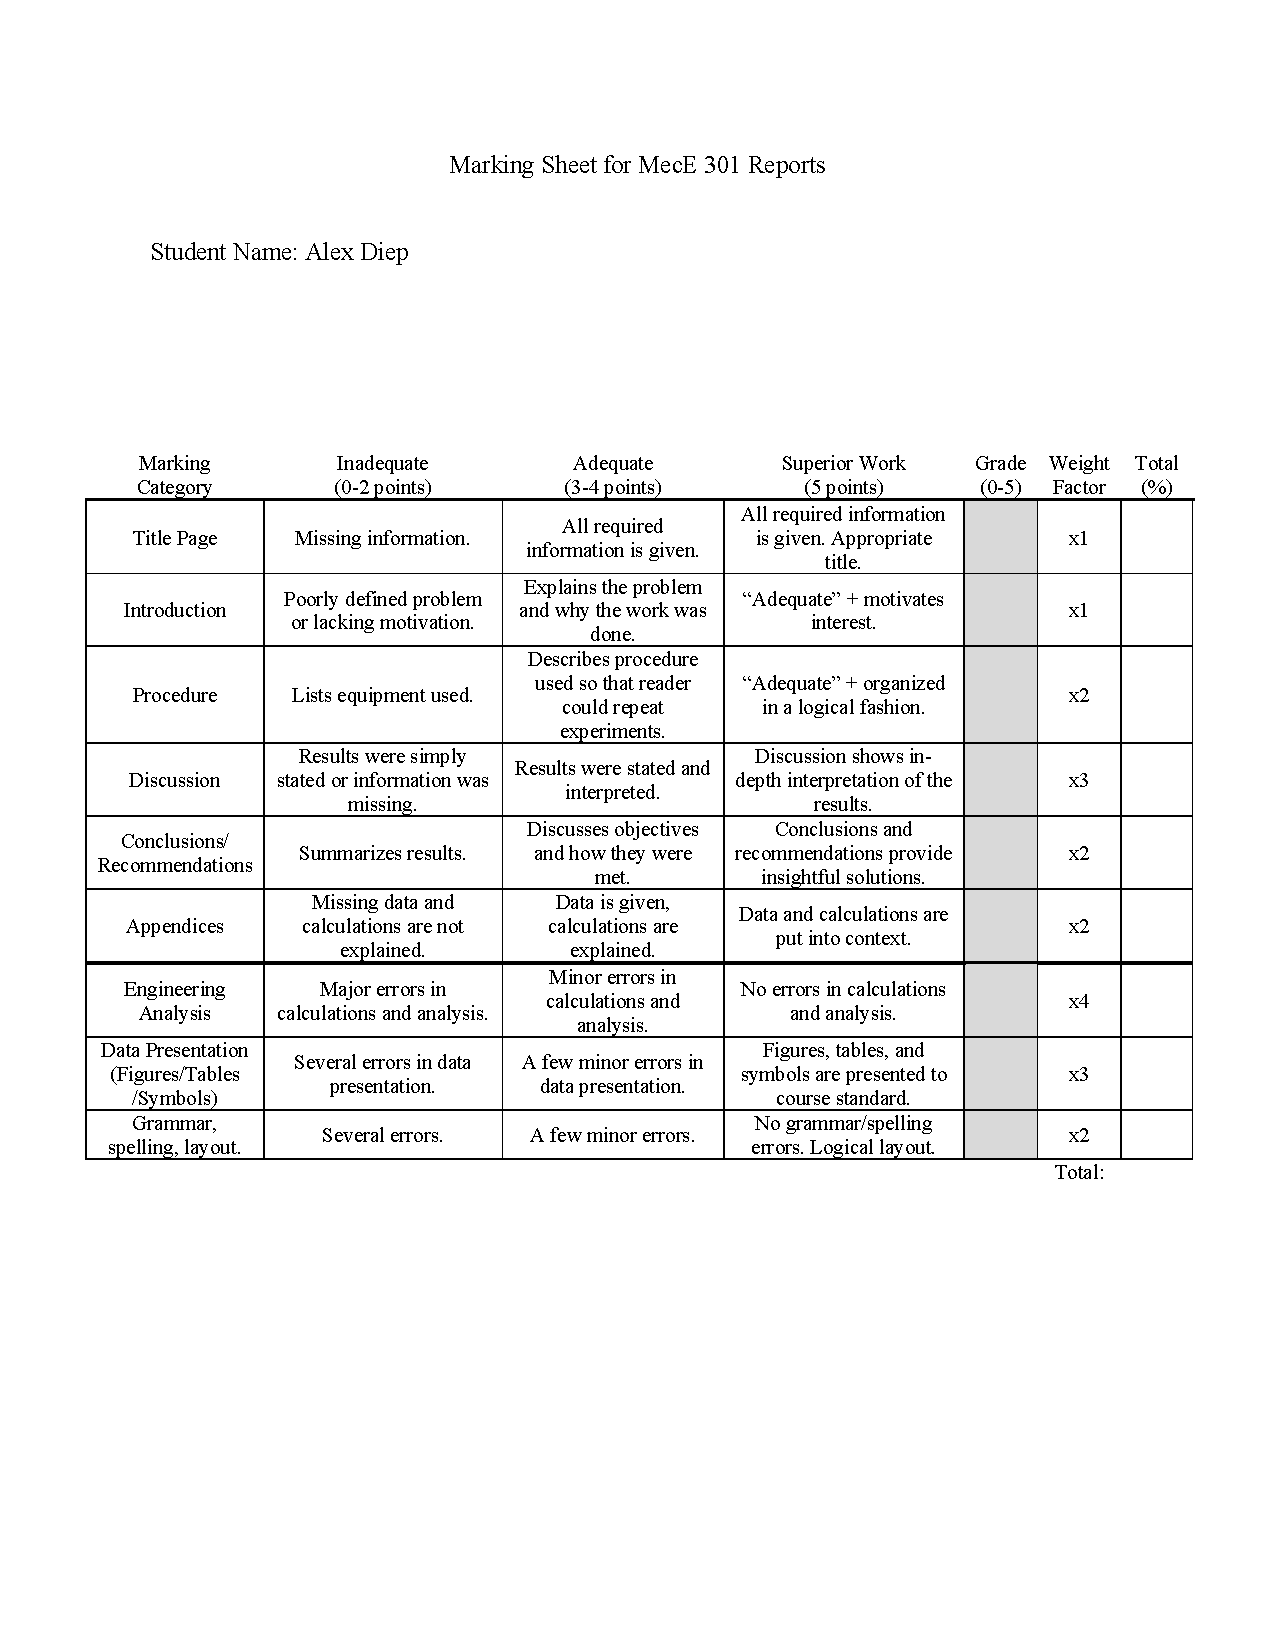
\includepdf[pages=-]{rubric.pdf}


\begin{titlepage}
    \centering
    \vspace*{2cm} % Adjust vertical spacing
    
    % Title
    \Huge {MEC E 301 \\Lab 2: Digital Measurement Techniques} \\
    \vspace{1cm} % Adjust vertical spacing
    
    % Author
    \Large by: Alex Diep \\
    \vspace{1cm} % Adjust vertical spacing

    % Date
    \Large Date: October 3, 2023 \\ % or manually specify a date
    \vspace{4cm} % Adjust vertical spacing

    % CCID and Student ID in smtaller font
    \normalsize CCID: abdiep \\
    \normalsize Student ID: 1664334 \\ 
    \normalsize Section: D21 \\
    
    \vfill % Fill vertical space
    
    % Additional content (e.g., university logo or other information)
    
\end{titlepage}
\renewcommand\arraystretch{1.5}

% Table of Contents (Hyperlinks set to locally black)
{
    \hypersetup{hidelinks}
    \tableofcontents
}
% use roman numerals for page numbers in table of contents
\pagenumbering{roman}

\newpage

% seperate page count for main matter
\pagenumbering{arabic}


\section{Introduction}

\noindent The primary objective of this lab is to investigate and familiarize elements of digital measurements such as 
word length (number of bits), quantization, resolution, conversion rates, sampling, accuracy, and signal conditioning through the use of an Arduino Uno. 
These concepts are important in signal processing and digital communications and familiarity with them is important for future development.



\section{Procedure}
% Requirements
% State the procedure followed in taking the data. The procedure should be organized 
% in the most concise, logical order; it does NOT need to be chronological. Use past 
% tense to tell the reader how you made the measurements. The reason for making each 
% measurement should also be given if necessary. e.g. "Stagnation pressure was measured 
% at 12 locations across the duct in order to determine average velocity". Include the make 
% and model number for important equipment used in the study. For MecE301 reports 
% this section is usually one or two paragraphs and one or two schematic figures. 
% Presenting, and referring to, a schematic diagram of the set-up saves words (and time) 
% and helps reader comprehension

\subsection{Equipment}
The following equipment was used to perform the experiment: Arduino Uno, MEC E 301 Shield, computer, oscilloscope, and jumper wires.

\subsection{Calibration}
\noindent A schematic of the experimental setup is shown in Figure [insert figure].
For extensive details on the calibration procedure, refer to the precis provided by the MEC E 301 course
All measurements were taken from the serial monitor of the Arduino IDE. During calibration, different circuit components 
and reference voltages were used to measure the voltage output of the PCB.

First, measuring voltages with a 5V reference voltage was performed. The \texttt{5V} and \texttt{GND} pins on the Arduino Uno were
connected to the \texttt{5V\_VIN} and \texttt{GND} pins on the PCB. The \texttt{A0} pin on the Arduino Uno was connected to the output pin,
\texttt{2.500V}. After uploading the sketch, ten values were recorded from the serial monitor. The \texttt{2.500V} output pin was then
swapped to \texttt{1.800V}, \texttt{1.024V}, and \texttt{0.102V} and ten values were recorded for each.

Next, measuring voltages with a 3.3V reference voltage was performed. The AREF jumper on the MEC E 301 Shield was inserted, connecting the
3.3V reference voltage to the AREF pin on the Arduino Uno. The code was modified to reflect the new reference voltage, \texttt{float voltage = sensorValue * (3.3 / 1024.0);}.
The voltages \texttt{2.500}, \texttt{1.800}, \texttt{1.024}, and \texttt{0.102} were measured again and ten values were recorded for each.

The next calibrations utilzied different circuit components. Connecting the output pin on the PCB to the \texttt{D10\_I}, \texttt{+/-10\_I}, and \texttt{X10\_I} pins on 
the MEC E 301 Shield allowed for the use of a voltage divider, [-10, 10]V range, and amplifier respectively. The \texttt{D10\_O}, \texttt{+/-10\_O}, and \texttt{X10\_O} 
pins on the MEC E 301 Shield were connected to the \texttt{A0} pin on the Arduino Uno. The calibration voltages \texttt{2.500}, \texttt{1.800}, \texttt{1.024}, and \texttt{0.102}
were measured again and ten values were recorded for each.

\subsection{Time Varying Voltage}
\noindent The \texttt{SINE\_OP} pin on the PCB was connected to the \texttt{A0} pin on the Arduino Uno. The code was modified to output a timestamp and 
voltage value and the baud rate was set to 115200. The serial monitor was opened and the voltage was recorded for 255 values. The values were 
copied into an Excel spreadsheet for analysis.


% \forceindent The following procedure was followed as outlined in the lab precis \cite{lab2precis}. First, the Arduino Uno was 
% connected to the computer and the Arduino IDE was opened. The Arduino IDE was used to upload the \texttt{AnalogReadSerial} after 
% modifying the code \texttt{float voltage = sensorValue * (5.0 / 1024.0);} to correct the decimal-to-number conversion. 
% An additonal line was added \texttt{Serial.println(voltage, 3)} to print the voltage to the serial monitor with 3 decimal places. 

% First, measuring voltages with a 5V reference voltage was performed. The \texttt{5V} and \texttt{GND} pins on the Arduino Uno were 
% connected to the \texttt{5V\_VIN} and \texttt{GND} pins on the PCB. The \texttt{A0} pin on the Arduino Uno was connected to the output pin,
% \texttt{2.500V}. After uploading the sketch, ten values were recorded from the serial monitor. The \texttt{2.500V} output pin was then
% swapped to \texttt{1.800V}, \texttt{1.024V}, and \texttt{0.102V} and ten values were recorded for each. 

% Next, measuring voltages with a 3.3V reference voltage was performed. The AREF jumper on the MEC E 301 Shield was inserted, connecting the 
% 3.3V reference voltage to the AREF pin on the Arduino Uno. The code was modified to reflect the new reference voltage, \texttt{float voltage = sensorValue * (3.3 / 1024.0);}.
% The voltages \texttt{2.500}, \texttt{1.800}, \texttt{1.024}, and \texttt{0.102} were measured again and ten values were recorded for each.

% % next was using voltage divider to measure voltages
% Next, measuring voltages with a voltage divider was performed. The output pin on the PCB was connected to the \texttt{D10\_I} on the MEC E 301 Shield.
% The \texttt{D10\_O} pin on the MEC E 301 Shield was connected to the \texttt{A0} pin on the Arduino Uno. The code was modified to reflect the new range 
% of voltages, \texttt{float voltage = sensorValue * (33.0 / 1024.0);}. The voltages \texttt{2.500}, \texttt{1.800}, \texttt{1.024}, and \texttt{0.102} 
% were measured again and ten values were recorded for each.

% % using -10 to 10 v range
% Next, measuring voltages with a -10V to 10V range was performed. The \texttt{+/-10\_I} was connected to the PCB output pin. The \texttt{+/-10\_O} pin on the MEC E 301 Shield
% was connected to the \texttt{A0} pin on the Arduino Uno. The code was modified to reflect the new range of voltages, \texttt{float voltage = sensorValue * (20.0 / 1024.0) - 10.0;}.
% The voltages \texttt{2.500}, \texttt{1.800}, \texttt{1.024}, and \texttt{0.102} were measured again and ten values were recorded for each.

% %using amplifier
% Voltage measurements with an amplifier was performed. The \texttt{X10\_I} pin on the MEC E 301 Shield was connected to the PCB output pin. The \texttt{X10\_O} pin on the MEC E 301 Shield
% was connected to the \texttt{A0} pin on the Arduino Uno. The code was modified to reflect the new range of voltages, \texttt{float voltage = sensorValue * (0.33 / 1024.0);}.
% The voltages \texttt{2.500}, \texttt{1.800}, \texttt{1.024}, and \texttt{0.102} were measured again and ten values were recorded for each.

% % pcb time varying voltage
% Time varying voltage measurements were performed. The \texttt{SINE\_OP} pin on the PCB was connected to the \texttt{A0} pin on the Arduino Uno. The code was modified to reflect the new range of voltages, 
% \texttt{float voltage = sensorValue * (3.3 / 1024.0);}. The code was modified to ouptut a timestamp and voltage value and the baud rate was set to 115200. The serial monitor was opened and the
% voltage was recorded for 255 values.



% % MecE 301 1
% % TEMPERATURE MEASUREMENT
% % Temperature measurement is perhaps the broadest area in engineering measurements. 
% % There are a wide range of sensors and instruments available that allow the measurement of 
% % temperature from cryogenic levels to that found in flames and higher. As always you should 
% % be aware of characteristics such as accuracy, resolution, linearity, usable range, response 
% % time, cost, etc. as well as the underlying principles of operation.
% % NOTE 1: This lab requires you to wire your own circuits. While you are wiring, make 
% % sure your Arduino is not powered on.
% % NOTE 2: Turn on the heater (Figure 5) now so the temperature is stable when you 
% % need to use it.
% % 1 TEMPERATURE SENSOR CALIBRATION
% % CAUTION! The water in the electrically heated water baths become extremely hot 
% % (up to 90 o
% % C). 
% % 1.1 EQUIPMENT - Sensor Calibration
% % The following is a list of the temperature sensors to be calibrated and the equipment used 
% % for the calibration.
% % • Electrically heated water baths with circulating pump. The temperature of each bath 
% % is measured with a 4-wire platinum RTD (cost ~$100). The accuracy of the RTD
% % and RTD meter is approximately 0.3 o
% % C
% % • Arduino Uno
% % • Type K thermocouple (~$1)
% % • Adafruit-AD8495 K-type thermocouple amplifier (~$8)
% % • Honeywell TD5A thermistor (~$5)
% % • Breadboard, jumper wires, and resistors
% % 1.2 PROCEDURE - Sensor Calibration
% % We’ll be using an Arduino, a Type-K thermocouple and thermistor to measure temperature. 
% % We’ll start by building circuits so that our Arduino can read a voltage output from the 
% % thermocouple and thermistor. 
% % The circuits will be built on a breadboard. A schematic of a breadboard is shown in 
% % Figure 1. The horizontal holes of the breadboard are electrically connected, but not across 
% % the middle divider. On each side of the board there are vertical columns which are 
% % electrically connected. These ‘bus strip’ are typically used to supply power and ground to 
% % the circuit. Connect the 5V pin of your Arduino to the “+” bus strip and the GND pin of 
% % your Arduino to the “–“ bus strip.
% % MecE 301 2
% % Figure 1: Schematic of breadboard. Source: computers.tutsplus.com
% % 1.2.1 Thermistor circuit
% % Build the circuit for the Honeywell TD5A thermistor which is found in Figure 2 of the 
% % TD5A data sheet (posted on eClass). The circuit is a simple ‘ballast’ circuit. Before 
% % building the circuit, disconnect the Arduino from your computer. This will prevent 
% % potential damage to the circuitry as you are building it. The resistance value of a resistor 
% % can be determined by the colour bands as shown in Figure 2. If you have a hard time reading 
% % the colours, you can measure the resistance with a multimeter.
% % Figure 2: Resistor colour codes
% % The voltage Vo shown on Figure 2 of the TD5A data sheet is an analog voltage which will 
% % change as the temperature of the thermistor changes. Connect this voltage to pin A0 of your 
% % MecE 301 3
% % Arduino. Connect the Arduino to your computer and open the built-in sketch 
% % ReadAnalogVoltage (File > Examples > 01.Basics > ReadAnalogVoltage).
% % In the void setup section add the line:
% % analogReference(EXTERNAL);
% % In the void loop section change the line: 
% % int sensorValue = analogRead(A0);
% % and change:
% % float voltage = sensorValue * (5.0 / 1023.0);
% % to 
% % float voltage = sensorValue * (3.3 / 1024.0);. 
% % Also, change the line:
% % Serial.println(voltage);
% % to 
% % Serial.println(voltage,3);
% % to make the serial monitor print out three digits.
% % Upload the code and warm up the thermistor with your fingers to verify the voltage 
% % increases as the thermistor warms. 
% % 1.2.2 Adafruit AD8495 circuit and Thermocouple (K Type)
% % (Information for the Adafruit AD8495: https://www.adafruit.com/products/1778)
% % The voltage output of typical thermocouple is on the order of microvolts which is too low 
% % for the Arduino to measure. Therefore, a thermocouple amplifier is used (Adafruit 
% % AD8495, Figure 3). This device amplifies the thermocouple voltage and it also provides a 
% % cold-junction reference so that the thermocouple outputs a voltage referenced to 0 o
% % C. The 
% % cold-junction reference is a silicon transistor similar to the one described in Section 3 of 
% % the lecture notes. The Adafruit AD8495 integrated circuit (IC) has a sensitivity of 5 mV/o
% % C, 
% % and the equation used to convert voltage output from the amplifier to temperature is given 
% % on the underside of the Adafruit (see Figure 3).
% % MecE 301 4
% % (a) (b)
% % Figure 3: Photos of (a) Adafruit AD8495, showing pin designations; (b) Underside of Adafruit showing 
% % voltage-temperature conversion equation.
% % Figure 4 is an image showing the wiring of the Arduino Uno, Adafruit AD8495, and the 
% % thermistor using the breadboard and supplied jumper wires, ready to use for temperature 
% % measurements. The AD8495 board has four pins: V+, GND, OUT, and GND. Connect the 
% % V+ pin to 5 V on the breadboard and both GND pins to ground on the breadboard. Connect 
% % the OUT pin to pin A1 on your Arduino. 
% % MecE 301 5
% % Figure 4: Photo of the Arduino Uno, Adafruit AD8495 Amplifier, thermistor circuit, and breadboard showing 
% % jumpers. 
% % Modify your existing Arduino code report the following to the serial port: i) thermistor
% % voltage, ii) the AD8495 voltage, and iii) convert the AD8495 voltage to temperature (see 
% % MecE 301 6
% % Figure 3 b). (For example, “Serial.print(value1,3); Serial.print(','); 
% % Serial.println(value2,3);” will write two values on a line delimited by a comma).
% % Add a line: delay(100); to your code so that the loop only executes every 100 ms. An 
% % example code is shown in Figure 5. Reconnect the Arduino to your computer. Upload the 
% % code and open the serial monitor. Check that the thermocouple is reporting temperatures 
% % near room temperature (~22 o
% % C). 
% % Figure 5. Example code for measuring the thermistor and thermocouple voltages and thermocouple 
% % temperature. 
% % MecE 301 7
% % 1.2.3 Water bath calibration
% % There are three water baths with temperatures at room temperature, 40 o
% % C, and 60 o
% % C. Place 
% % your thermistor and thermocouple in a water bath and wait for their temperatures to 
% % stabilize (try to suspend them in the water rather than having them touch the bottom or 
% % sides of the container). Then record approximately 50 measurements for each device (i.e. 
% % cut-paste 50 values from the serial monitor into Excel) and record the water bath 
% % temperature. (You can “pause” the serial monitor by unchecking the “Autoscroll” check 
% % box so make it easier to cut-paste). Repeat this procedure for all the water baths.
% % Plot the calibration data for the thermistor in Excel and fit it with a straight line to get the 
% % correlating function. Enter this correlating function into your Arduino code so that you 
% % report the thermistor temperature to the serial monitor. Be sure to enter this correlating 
% % function so that your measurements in the transient tests (below) are in units of 
% % temperature.
% % 2 TRANSIENT RESPONSE
% % 2.1 EQUIPMENT - Transient Response
% % The transient temperature response of the thermocouple and thermistor is investigated 
% % using the equipment used above and 
% % • A heater (Figure 5)
% % • A beaker of room temperature water.
% % NOTE: ensure that your Arduino code reports temperature (not voltage), to the serial 
% % monitor, for both the thermistor and thermocouple.
% % 2.2 PROCEDURE - Transient Response
% % Turn on the heater (Figure 5) if not already on. Modify your Arduino code so that you also 
% % display the time in the serial monitor: if you use Serial.print(micros()); the 
% % time in microseconds will be printed. Your code should write one line which contains the 
% % time and both temperatures (e.g. time,Temp1,Temp2). Also set the loop delay to 1 second 
% % (i.e. use delay(1000); in your loop). Turn on the Arduino serial monitor and display 
% % the time and temperatures of the thermistor and thermocouple. Place the thermistor and 
% % thermocouple in the heater and allow them to come to equilibrium (this might take about 5
% % minutes for the thermistor). Once the temperatures are stable, remove the devices from the 
% % heater as quickly as possible to room temperature air and allow them to cool (keep the 
% % devices stationary as they cool and do not blow on them). Once the temperatures have 
% % stabilized, save the data by cut-pasting it to Excel. Select data starting from just before you 
% % removed the devices to the time the devices had cooled to room temperature (again, 
% % unchecking the “AutoScroll” button is useful). Plot the data.
% % MecE 301 8
% % Figure 5: Heater used for determining time constant of thermocouple and thermistor.
% % Fill the small Petri dish with some water and repeat this experiment using the water to cool 
% % the devices. This time set your loop delay to 10 milliseconds (i.e. use delay(10); in 
% % your loop).
% % Show your data to the teaching assistant before leaving the lab.
% % MecE 301 9
% % 3 REPORT
% % The purpose of the report is to compare the accuracy, resolution (all in terms of o
% % C), and 
% % time constant of the thermocouple and thermistor. When writing your report and presenting 
% % your work, be sure to present/include figures, tables, equations, and assumptions required 
% % to fully detail the answers to the questions below. Follow MecE301 guidelines for tables 
% % and figures.
% % Answer the following:
% % 1) Thermistor: Determine the accuracy and resolution of the thermistor. To find the 
% % resolution of a device divide the resolution of the A/D converter by the sensitivity of the 
% % device (See Section 2 in the Digital lecture notes). Mention any recommendations you 
% % might have for increasing the resolution of the measurement systems.
% % 2) Thermocouple: Determine the accuracy and resolution of the thermocouple. Do this for 
% % two cases: (1) for your temperature measurements obtained by using the Adafruit
% % conversion equation for voltage to temperature (stamped on the Adafruit); and (2) for your 
% % measurements based on a new correlating function that you determine by fitting a linear 
% % correlating function to voltage versus the reference temperature. Comment on which case 
% % (1 or 2) led to the best accuracy, and state why.
% % 3) Determine the time constant of the devices in the two systems (room temperature air and 
% % room temperature water) using the data collected from the transient tests. When you 
% % removed the devices from the heater and placed them in room temperature air or water you 
% % created a step-change for the devices. The devices are first-order systems and the firstorder response to a step change is,
% % (1)
% % where t is the time, t is the time constant, T is the temperature at time t, T0 is the initial 
% % temperature at t=0 (i.e. the time you removed the devices from the heater, it is constant and 
% % is not a variable in the equation), and is the temperature once the system has reached 
% % its new steady-state value after the step change (it is constant and is not a variable in the 
% % equation). 
% % To calculate the time constants, use chi-squared minimization to fit Eq 1 to your 
% % experimental data. Examples on how to use chi-squared minimization in Excel is shown 
% % here: 
% % http://web.chem.ucsb.edu/~laverman/Chem116/PDF116CL/Solver.pdf
% % https://jkp-ads.com/articles/leastsquares.asp
% % https://www.youtube.com/watch?v=Ewp5CF5ba_w
% % (Note: Don’t use the equations given in the examples, use Equation 1 for your fit.)
% % T =T∞ +(T0 −T∞ )e
% % −t
% % τ
% % T∞
% % MecE 301 10
% % The time constant of a temperature measurement device is a function of the rate of heat 
% % transfer to/from the sensor. Discuss why the time constants are different between devices 
% % (i.e. thermocouple vs thermistor) and between the surroundings (i.e. air vs water).
% \section{Procedure}
% % 3. Procedure
% % State the procedure followed in taking the data. The procedure should be organized 
% % in the most concise, logical order; it does NOT need to be chronological. Use past 
% % tense to tell the reader how you made the measurements. The reason for making each 
% % measurement should also be given if necessary. e.g. "Stagnation pressure was measured 
% % at 12 locations across the duct in order to determine average velocity". Include the make 
% % and model number for important equipment used in the study. For MecE301 reports 
% % this section is usually one or two paragraphs and one or two schematic figures. 
% % Presenting, and referring to, a schematic diagram of the set-up saves words (and time) 
% % and helps reader comprehension.

% \subsection{Equipment}
% \noindent The following equipment was used to perform the experiment: Arduino Uno, MEC E 301 Shield, laptop, USB cable, breadboard,
% jumper wires, $\qty{5110}{\ohm}$ resistor, ANOVA sous vide precision cooker, large container for water bath, heater, petri dish, 
% 4-wire platinum RTD, Type K thermocouple, Adafruit-AD8495 K-type thermocouple amplifier, and Honeywell TD5A thermistor.

% \subsection{Setup}
% \noindent The circuit shown in Figures \ref{fig:TD5A_circuit} and \ref{fig:lab_manual_circuit} were built on a breadboard. The example code \textit{ReadAnalogVoltage} 
% was modified to read the voltage from the thermistor and thermocouple. The equation for the thermocouple, found on the underside of the Adafruit AD8495, 
% was used to convert the voltage to temperature.

% Three water baths were prepared. The first water bath was filled with room temperature water. The second and third water baths were filled with water 
% with the ANOVA sous vide precision cooker set to $\qty{40}{\celsius}$ and $\qty{60}{\celsius}$, respectively. Half an hour was given for the water baths to reach
% the desired temperature. 

% \subsection{Calibration}
% \noindent The calibration of the both the thermistor and thermocouple were performed by placing the devices in the water baths and allowing them to reach
% equilibrium. Fifty temperature and voltage measurements were recorded at equilibrium for each water bath. 

% \subsection{Transient Response}
% The thermistor and thermocouple were placed in the heater until they reached equilibrium, about five minutes. The devices were then removed from the heater
% and allowed to cool to room temperature in air. The temperature, voltage, and timestamps were recorded every second. 

% Again, the thermistor and thermocouple were placed in the heater until they reached equilibrium. Water was poured into a petri dish.
% The devices were then removed from the heater and submerged in the water in the petri dish. The temperature, voltage, and timestamps were recorded 
% every ten milliseconds. 
\section{Results and Discussion}
\subsection{Calibration}
\begin{table}[h]
    \centering
    \caption{Accuracy, repeatability, and resolution of the thermistor and thermocouple.}
    \label{tab:accuracy}
    \begin{tabular}{lccc}
        \toprule
        & Thermistor & Thermocouple & Thermocouple with Linear Fit \\
        \midrule
        Accuracy & $\qty{2.2}{\celsius}$ & $\qty{1.8}{\celsius}$ & $\qty{0.8}{\celsius}$ \\
        Repeatability & $\qty{3.3}{\celsius}$ & $\qty{1.3}{\celsius}$ & $\qty{1.4}{\celsius}$ \\
        Resolution & $\qty{1.1}{\celsius}$ & $\qty{0.6}{\celsius}$ & $\qty{0.6}{\celsius}$ \\
        \bottomrule
    \end{tabular}
\end{table}
\noindent The thermistor was the worst performing device in terms of accuracy and repeatability. There are several ways to improve the resolution of the 
thermistor. The equation for resolution is given by
\begin{equation}
    Resolution = \frac{\Delta V_{\text{fs}}}{2^{n}\times Sensitivity} \label{eq:resolution}
\end{equation}
where $\Delta V_{\text{fs}}$ is the full-scale voltage and $n$ is the number of bits.

From (\ref{eq:resolution}), there are three recommendations to increase the resolution of the thermistor. The first is to utilize an A/D 
with a more bits. The second is to increase the sensitivity of the device by using a different material such as platinum. The third is to 
decrease the full-scale voltage by using an amplifier. The effects of saturation may need to be taken into consideration with the usage of \
an amplifier.

The thermocouple voltage data was processed in two ways. First the Adafruit conversion equation was used to convert the voltage to temperature.
Second, a linear fit was performed on the calibration data to convert the voltage to temperature. The accuracy, repeatability, and resolution
of the thermocouple with the Adafruit conversion equation and the linear fit are shown in Table \ref{tab:accuracy}. 

The thermocouple with the linear fit has a higher accuracy and repeatability than with the Adafruit conversion equation. This is because the
linear fit is based on the calibration data, which is more accurate than the Adafruit conversion equation. Variation in manufacturing of the
thermocouple and the Adafruit AD8495 amplifier could contribute to the lower accuracy of the conversion equation.

\subsection{Transient Response}
% Air		Water	
% Thermistor	Thermocouple	Thermistor	Thermocouple
% tau	18.69803057	18.02662691	0.373547583	0.225033996

\begin{table}[h]
    \centering
    \caption{Time constants of the thermistor and thermocouple in air and water.}
    \label{tab:time_constants}
    \begin{tabular}{lcccc}
        \toprule
        & \multicolumn{2}{c}{Air} & \multicolumn{2}{c}{Water} \\
        \cmidrule(lr){2-3} \cmidrule(lr){4-5}
        & Thermistor & Thermocouple & Thermistor & Thermocouple \\
        \midrule
        $\tau$ & $\qty{18.698}{\second}$ & $\qty{18.027}{\second}$ & $\qty{0.374}{\second}$ & $\qty{0.225}{\second}$ \\
        \bottomrule
    \end{tabular}
\end{table}
\noindent The time constant is a function of the rate of heat transfer to/from the sensor. The higher rate of heat transfer, the lower the time constant. 
Since water has a higher convection coefficient than air, the time constants are expected to be lower in water than in air. This agrees with the experimentally 
determined time constant values where for both the thermistor and thermocouple, the time constants in water are lower than in air by about two orders of magnitude.

Thermistors are made of ceramic-like materials whereas thermocouples are made of metal. Metals have free electrons resulting in higher thermal
conductivity than ceramics. Since the time constant decreases with increasing heat transfer, the thermocouple is expected to have a lower time constant than the
thermistor. This agrees with the experimentally determined time constant values where the thermocouple has a lower time constant than the thermistor for
both air and water.

The first order fit was a good approximation of the experimental data. The first order $\chi^2$ fit was appropriate for the step response to the system. 
Figures \ref{fig:thermistor_transient_air}, \ref{fig:thermocouple_transient_air}, \ref{fig:thermistor_transient_water}, and 
\ref{fig:thermocouple_transient_water} show the experimental data and the first order fit. 


\section{Conclusion}
\label{sec:conclusion}

\noindent The calibration section of the lab highlighted important concepts such as quantization, the trade-off between resolution and range, and the importance 
of a known reference voltage. The Arduino Uno was used to measure the voltage across different circuit components and reference voltages, and their 
impact on resolution, accuracy, and range was observed. The time varying voltage section of the lab highlighted the importance of sampling rate and 
resolution. Hands-on experience with an oscilloscope was obtained, and measurements were compared to the Arduino Uno. The Arduino Uno was able to
somewhat agree with the much more expensive oscilloscope. Increasing the sample rate and resolution of the Arduino Uno would allow for better agreement
with the oscilloscope.

% \newpage
% %\bibliographystyle{IEEEtran}
% %\bibliography{citations.bib}
% %\bibliography{}

\newpage
\appendix
\renewcommand\thefigure{\thesection.\arabic{figure}}    
\renewcommand\thetable{\thesection.\arabic{table}}
\section{Figures}
\label{sec:figures}
\subsection{Schematic of the system}
asd

\subsection{Plots of Time-Varying Signals}
\begin{figure}[h]
    \centering
    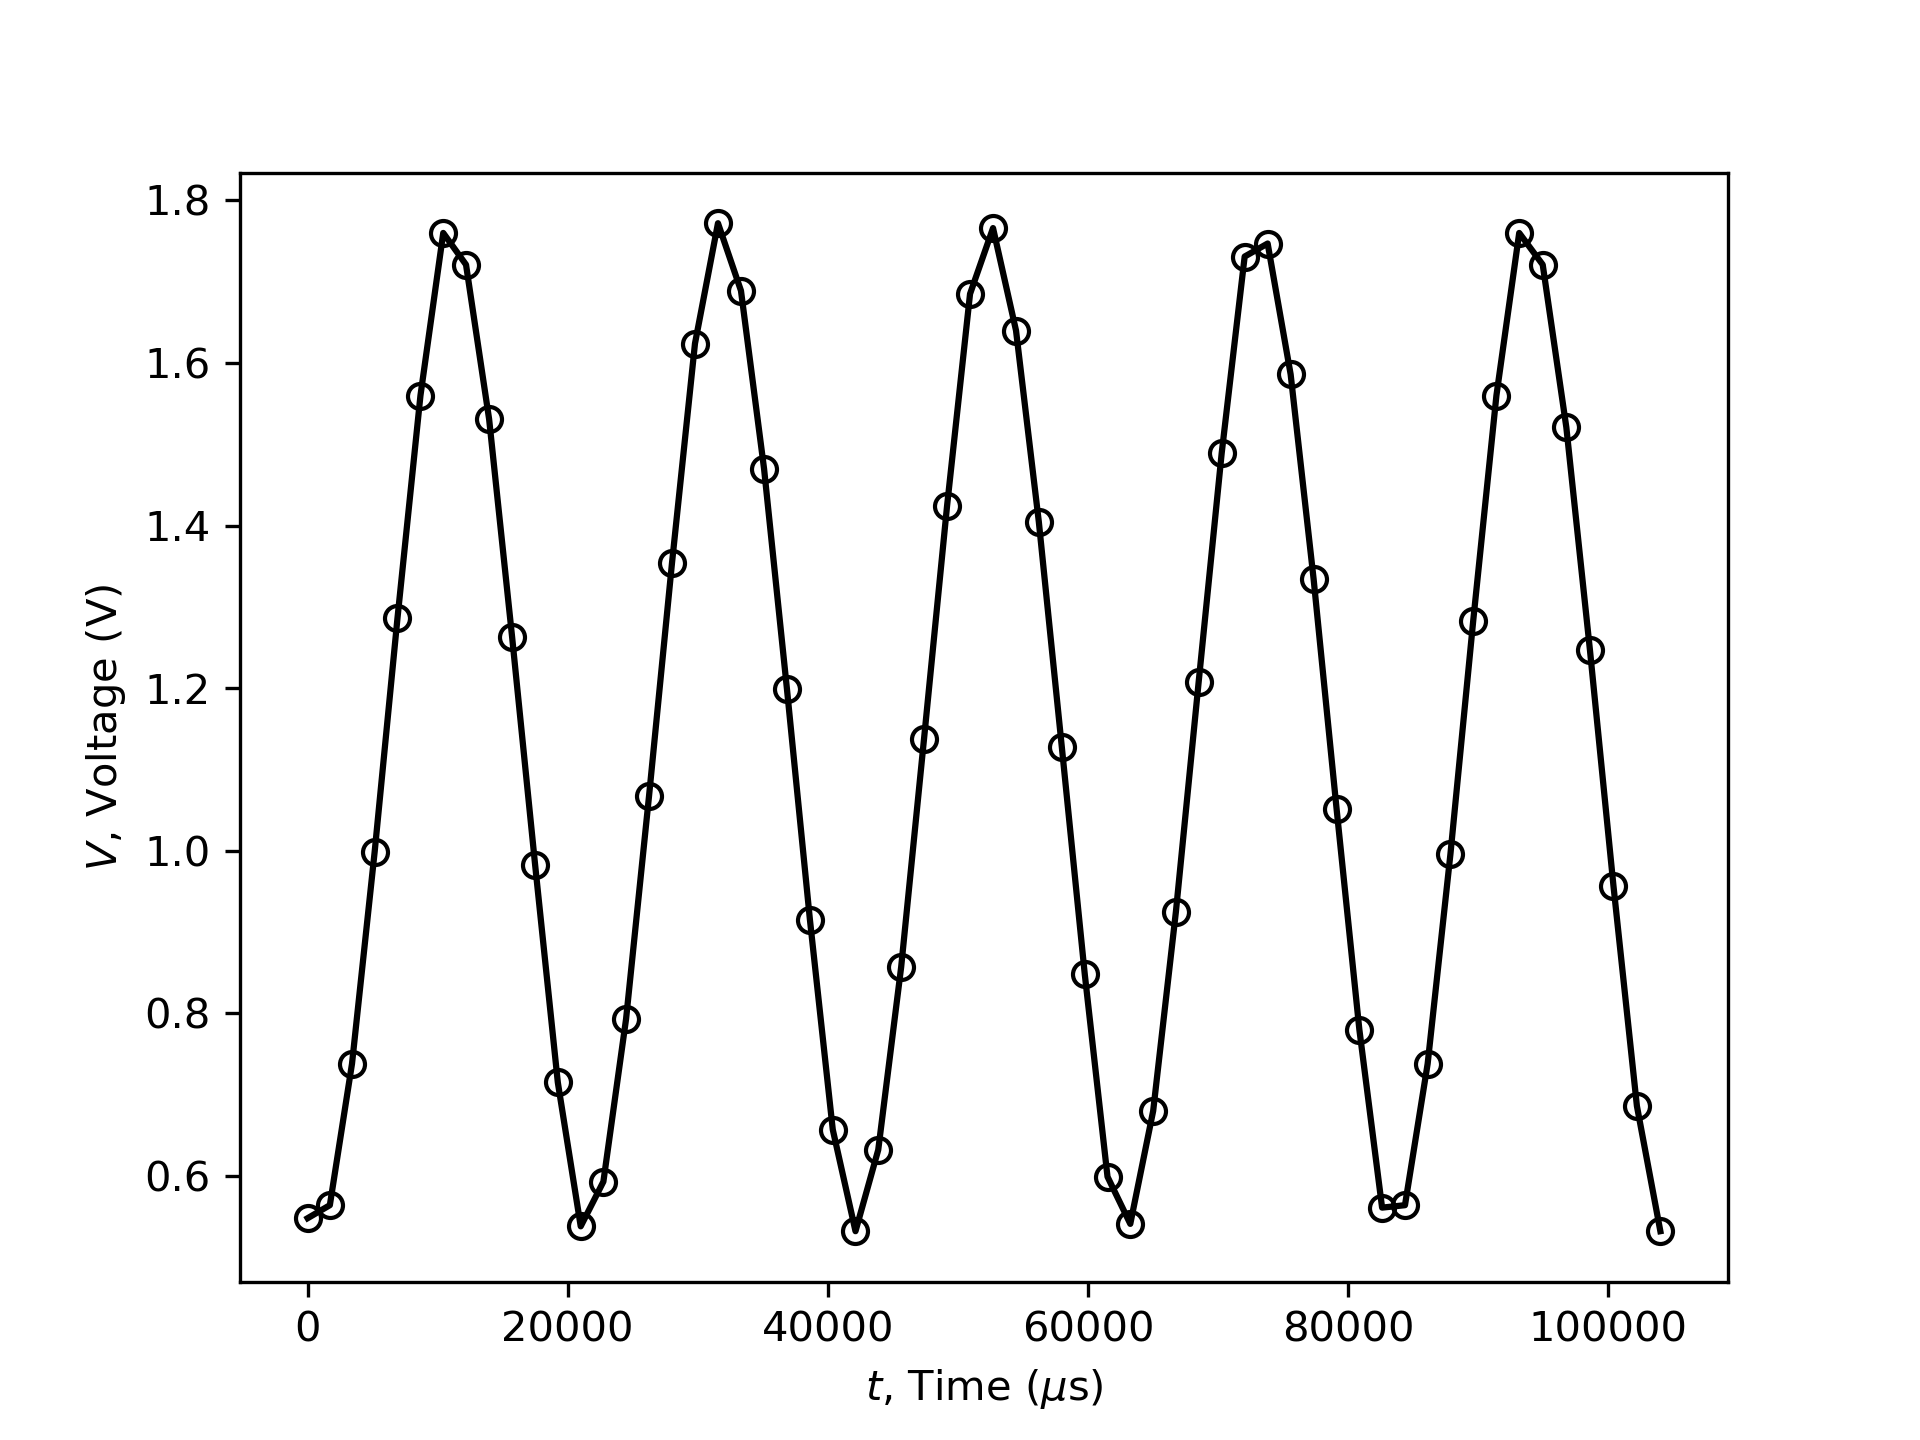
\includegraphics[width=0.5\textwidth]{Sections/Figures/10bit.png}
    \caption{Time varying signal of PCB 18 Measured with 10-bit ADC of the Arduino Uno}
    \label{fig:10bit}
\end{figure}

\begin{figure}[h]
    \centering
    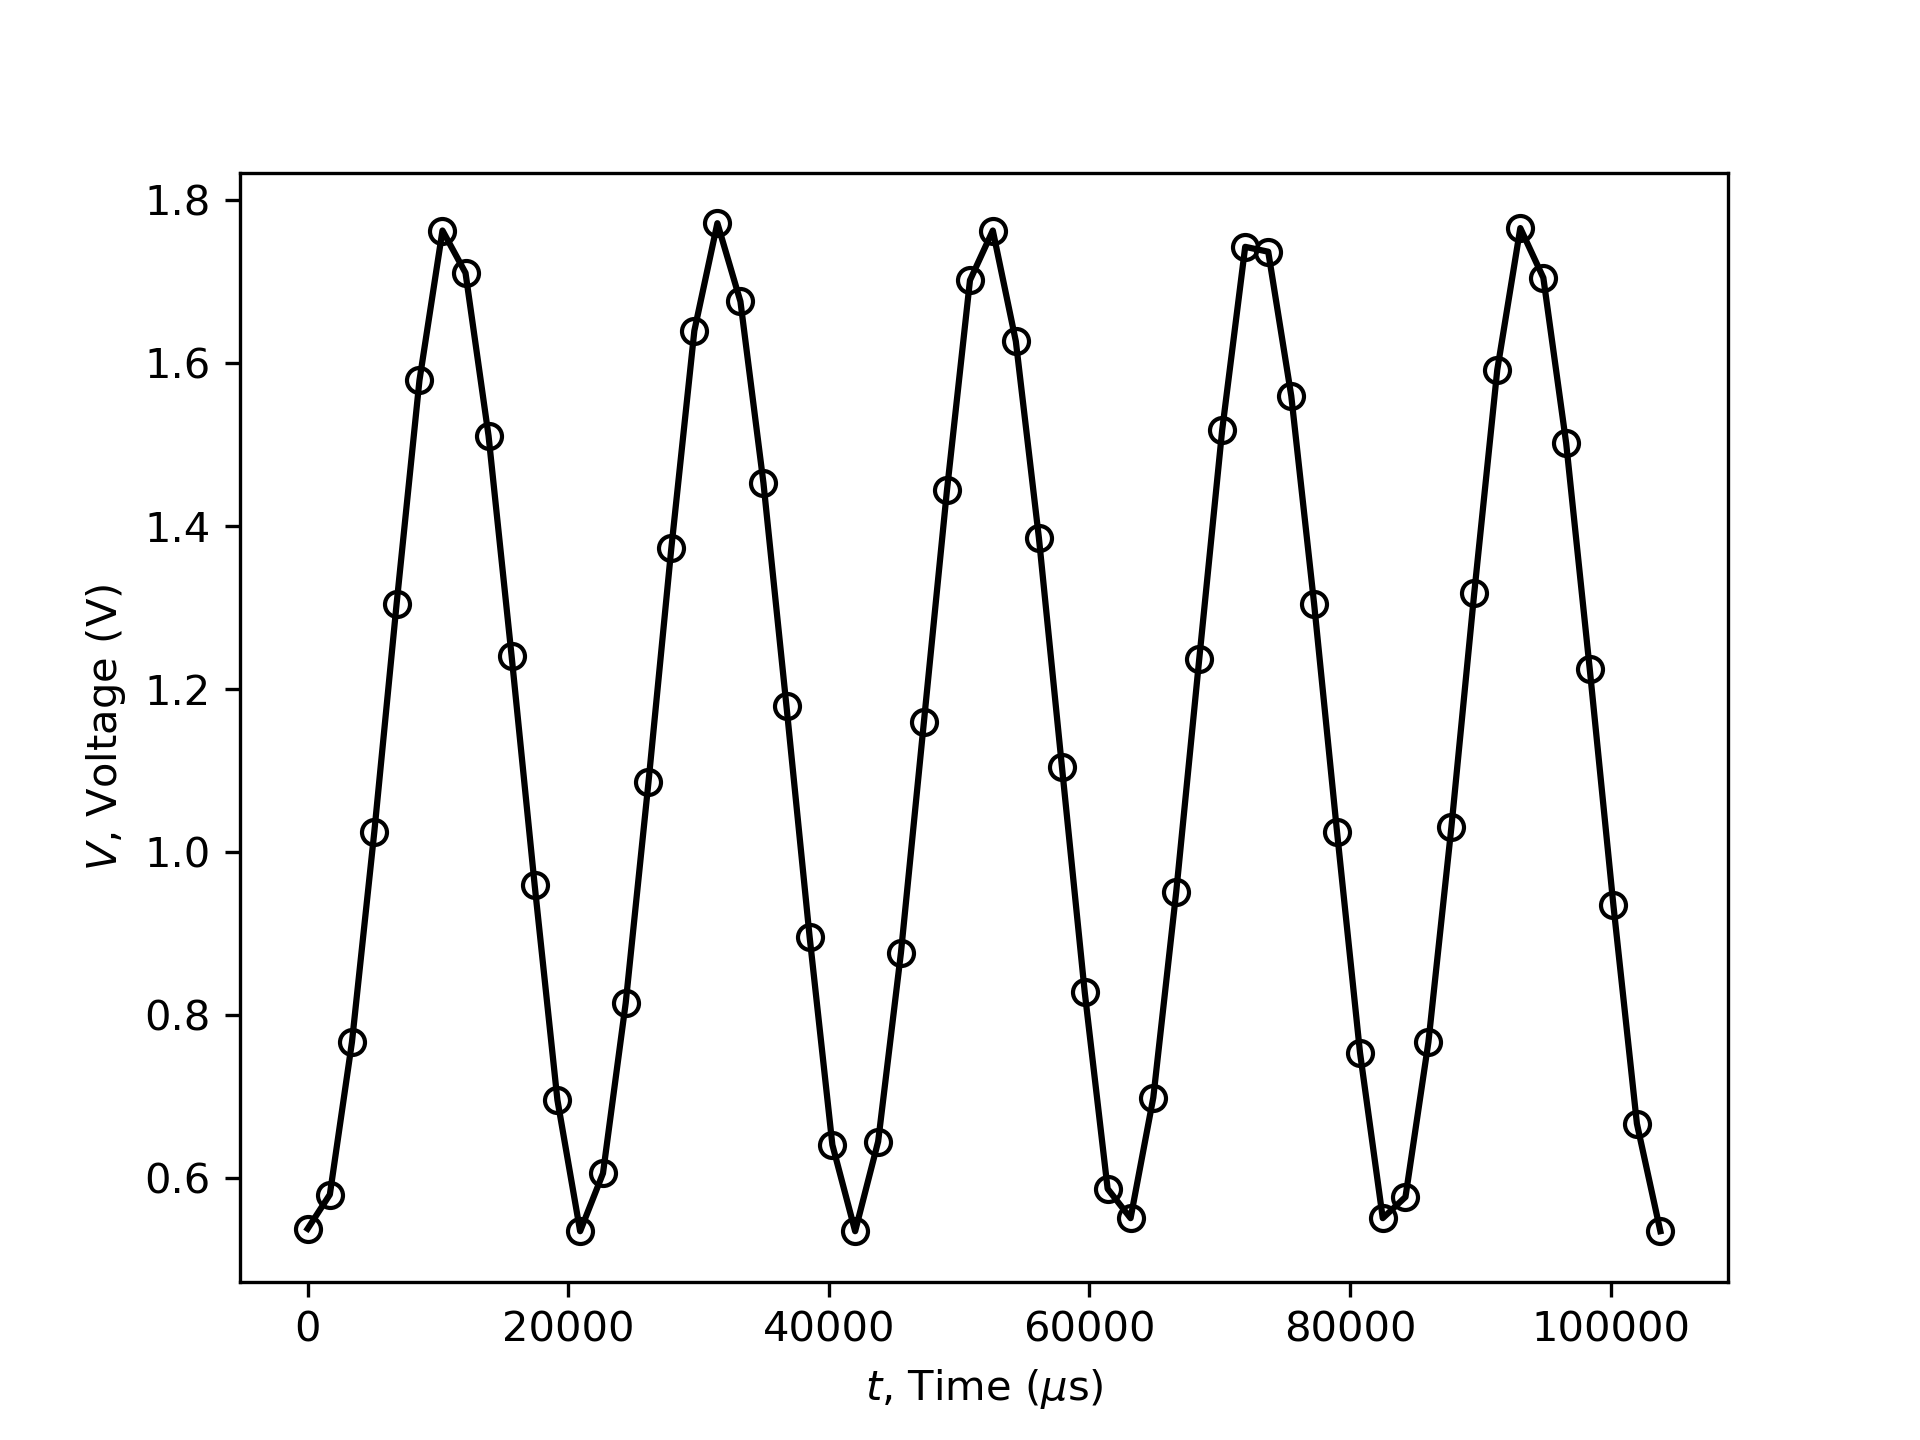
\includegraphics[width=0.5\textwidth]{Sections/Figures/5bit.png}
    \caption{Time varying signal of PCB 18 Measured with 5-bit ADC of the Arduino Uno}
    \label{fig:5bit}
\end{figure}
\newpage
\section{Appendix: Arduino Uno Calibration Results}
%\label{sec:appendix-arduino-calibration}
\begin{table}[ht]
    \caption{Range, Resolution, Repeatability, Accuracy, and Manufacturer's Accuracy for Various Ranges of the Arduino Uno}
    \label{tab:arduino-accuracy}
    \centering
    \small
    \begin{tabular}{lccccc}
        \toprule
        Arduino Config. & Range & Resolution & Repeatability & Acc. & Manuf. Acc. \\
        & (V) & (mV/LSB) & ($\pm$mV) & ($\pm$mV) & ($\pm$mV) \\
        \midrule
        5V Ref. & 0.000 - 5.000 & 4.883 & 44.00 & 54.00 & 9.766 \\
        3.3V Ref. & 0.000 - 3.300 & 3.223 & 4.000 & 17.00 & 6.445 \\
        3.3V Ref., 10x VDiv & 0.00 - 33.00 & 32.23 & 32.00 & 83.00 & 64.45 \\
        3.3V Ref., [-10, 10]V & -10.00 - 10.00 & 19.53 & 0.000 & 24.00 & 39.06 \\
        3.3V Ref., 10x Amp. & 0.000 - 0.330 & 0.3223 & 0.000 & 0.000 & 0.6445 \\
        \bottomrule
    \end{tabular}
\end{table}
\newpage
\section{Appendix: Arduino Uno Accuracy}
\label{sec:appendix-arduino-accuracy}
Table \ref{tab:arduino-accuracy-appendix} summarizes the range, resolution, repeatability, accuracy, and manufacturer's accuracy for various ranges of the 
Arduino Uno. Sample calculations for the 5V reference voltage are shown below. Note, the manufacturer's accuracy is $\pm$ 2 LSBs.

\begin{align*}
    \text{Resolution} &= \frac{V_{\text{ru}} - V_{\text{rl}}}{2^n} \\
    &= \frac{5.000 - 0.000}{2^{10}} \\
    &= \boxed{\qty[per-mode=symbol]{4.883}{\milli\volt\per\LSB}} \\
    \text{Repeatability} &= \max({\text{Max Deviation}}) \\
    &= \max(\langle 5.00, 0.00, 9.00, 44.00 \rangle) \\
    &= \boxed{\qty{44.00}{\milli\volt}} \\
    \text{Accuracy} &= \max({\text{Deviation}}) \\
    &= \max\left(
        \tiny	
        \begin{bmatrix}
            -0.009 & -0.009 & -0.009 & -0.009 & -0.009 & -0.009 & -0.009 & -0.009 & -0.004 & -0.009 \\
            0.001 & 0.001 & 0.001 & 0.001 & 0.001 & 0.001 & 0.001 & 0.001 & 0.001 & 0.001 \\
            0.016 & 0.021 & 0.012 & 0.016 & 0.012 & 0.012 & 0.016 & 0.016 & 0.012 & 0.016 \\
            0.02 & 0.024 & 0.02 & 0.024 & 0.01 & 0.02 & \textbf{0.054} & 0.024 & 0.034 & 0.02 \\
        \end{bmatrix}
    \right) \nonumber \\
    &= \boxed{\qty{54.00}{\milli\volt}}\\
    \text{Manuf. Acc.} &= \qty{2}{\LSB} \times \text{Resolution} \\
    &= \boxed{\qty{9.766}{\milli\volt}}
\end{align*}

For significant figures, since the range is given to 3 decimal places, the resolution is given to 3 decimal places, more often
than not, the number of significant figures is 4. This is because addition and subtraction do not take into account the number of significant figures
but rather the number of decimal places.

\begin{table}[ht]
    \caption{Range, Resolution, Repeatability, Accuracy, and Manufacturer's Accuracy for Various Ranges of the Arduino Uno}
    \label{tab:arduino-accuracy-appendix}
    \centering
    \small
    \begin{tabular}{lccccc}
        \toprule
        Arduino Config. & Range & Resolution & Repeatability & Acc. & Manuf. Acc. \\
        & (V) & (mV/LSB) & (mV) & (mV) & (mV) \\
        \midrule
        5V Ref. & 0.000 - 5.000 & 4.883 & 44.00 & 54.00 & 9.766 \\
        3.3V Ref. & 0.000 - 3.300 & 3.223 & 4.000 & 17.00 & 6.445 \\
        3.3V Ref., 10x VDiv & 0.00 - 33.00 & 32.23 & 32.00 & 83.00 & 64.45 \\
        3.3V Ref., [-10, 10]V & -10.00 - 10.00 & 19.53 & 0.000 & 24.00 & 39.06 \\
        3.3V Ref., 10x Amp. & 0.000 - 0.330 & 0.3223 & 0.000 & 0.000 & 0.6445 \\
        \bottomrule
    \end{tabular}
\end{table}
\newpage
\section{Appendix: Derivation of Resolution}
\label{sec:appendix-resolution}
\noindent The trade-off between resolution and range is that as the range increases, the resolution decreases. This is because the number of bits
available to represent the range is fixed. For example, the Arduino Uno has 10 bits to represent the range of voltages. This means that the
Arduino Uno can represent $2^{10} = 1024$ different voltages. If the range is 0 to 5V, then the resolution is 4.883mV/LSB. If the range is
0 to 10V, then the resolution is 9.766mV/LSB. 

\noindent This can be shown mathematically. Then the resolution is given by:
\[
\begin{aligned}
    \text{Resolution} &= \frac{V_{\text{ru}} - V_{\text{rl}}}{2^n} \\
\end{aligned}
\]
Let us assume the upper range $V_{\text{ru}}$ and lower range $V_{\text{rl}}$ are both multiplied by a factor of $k$.
\[
\begin{aligned}
    \text{Resolution'} &= \frac{kV_{\text{ru}} - kV_{\text{rl}}}{2^n} \\
    &= \frac{k(V_{\text{ru}} - V_{\text{rl}})}{2^n} \\
    &= k \text{Resolution} \\
\end{aligned}
\]
\newpage
\section{Appendix: Voltage Source Accuracy}
\label{sec:appendix-voltage-source-accuracy}

\noindent The accuracy of the voltage source is 0.05\%. A table deviation from the true value is shown below.
\begin{table}[h]
    \centering
    \caption{Deviation from True Value for Voltage Source with 0.05\% Accuracy}
    \begin{tabular}{cc}
        \toprule
        Voltage & Deviation from True Value \\
        (V) & (mV) \\
        \midrule
            0.102 & 0.051  \\
            1.024 & 0.512  \\
            1.800 & 0.900    \\
            2.500 & \textbf{1.250}  \\
        \bottomrule
    \end{tabular}
\end{table}

\noindent As one can see, the voltage source deviation is 10x smaller than the accuracy of the Arduino Uno. This means that the voltage 
source is a suitable reference voltage for the Arduino Uno.

\begin{table}[h]
    \centering
    \caption{Accuracy of Voltage Source Compared to Arduino Uno}\
    \label{tab:voltage-source-accuracy}
    \begin{tabular}{lc}
        \toprule
        Configuration & Accuracy  \\
                          & (mV)      \\
        \midrule
    Voltage Source        & 1.250      \\
    5V Ref.~              & 54.00     \\
    3.3V Ref.~            & 17.00     \\
    3.3V Ref., 10x VD     & 83.00     \\
    3.3V Ref., [-10, 10]V & 24.00     \\
    3.3V Ref., 10x Amp.~  & 0.000    \\
    \bottomrule
    \end{tabular}
\end{table}
\newpage
\section{Appendix: Circuit Component Accuracy}
\label{sec:appendix-circuit-component-accuracy}
Below is a table of the additional error from the voltage divider, voltage scaler, and amplifier. The error is calculated by multiplying the voltage by 1\%.

\begin{table}[h]
    \centering
    \caption{Additional Error from Voltage Divider, Voltage Scaler, and Amplifier}
    \begin{tabular}{cc}
        \toprule 
        Voltage & Error \\
        (V) & ($\pm$mV) \\
        \midrule
    0.102 & 1.020  \\
    2.500 & 25.00 \\
    \bottomrule
    \end{tabular}
\end{table}
\newpage
\section{Time-Varying Voltage Measurements}
\label{sec:appendix-time-varying-voltage-measurements}

\noindent Below in Table \ref{tab:time-varying-voltage-mean-measurements} are the nominal measurements for the time-varying voltage for the 10-bit and 5-bit ADCs.
\begin{table}[h]
    \centering
    \caption{Nominal Measurements of Time-Varying Voltage}
    \label{tab:time-varying-voltage-mean-measurements}
    \begin{tabular}{lccc}
      \toprule
           & \multicolumn{3}{c}{Mean Measurements of Time-Varying Voltage} \\
    \cmidrule{2-4}
           & Frequency & Peak to Peak & Mean Voltage       \\
           & (Hz)      & (V)          & (V)           \\
    \midrule
    10-bit & 47.266  & 1.217        & 1.135         \\
    5-bit  & 47.372  & 1.2194       & 1.144         \\
    Oscilloscope & 48.54 & 1.28 & 1.17 \\
   \bottomrule
    \end{tabular}
\end{table}
\subsection{Mean Sample Calculation}
\noindent The mean voltage for the 10-bit and 5-bit ADCs was calculated using Excel using the \texttt{=AVERAGE()} function across 5 cycles, which was
approximately 60 data points. 

\subsection{Time-Varying Voltage Period Measurements}

\noindent Below is a table of the time-varying period measurements for the 10-bit and 5-bit ADCs. 
\begin{table}[h]
    \centering
    \caption{Time-Varying Period Measurements for 10-bit and 5-bit ADCs}
    \begin{tabular}{lcccccc}
    \toprule
       & \multicolumn{5}{c}{Period ($\mu$s)}    \\
    \cmidrule{2-6}
       & Cycle 1    & Cycle 2   & Cycle 3   & Cycle 4   & Cycle 5    \\
    \midrule
    10-bit & 21000 & 21132 & 21132 & 21124 & 21400  \\
    5-bit  & 20912 & 21104 & 21136 & 21096 & 21304  \\
    \bottomrule
    \end{tabular}
\end{table}

\noindent \textbf{Obtaining the nominal value (mean)}, standard deviation, and T-distribution inverse was done through Excel. The mean was calculated using the \texttt{=AVERAGE()} function 
across 5 cycles, which was approximately 60 data points. The standard deviation was calculated using the \texttt{=STDEV.S()} function. 
The T-distribution inverse was calculated using the \texttt{=T.INV()} function, where $\alpha = 0.05$ and $n = 5$. The results are shown in Table 
\ref{tab:time-varying-period-uncertainty-measurements}.

\begin{table}[h]
   \centering
   \caption{Time-Varying Period Uncertainty Measurements for 10-bit and 5-bit ADCs}
   \label{tab:time-varying-period-uncertainty-measurements}
   \begin{tabular}{lcccccc}
      \toprule
      & Nominal Value & STDEV & T-Inv & $P_x$ \\
      & ($\mu$s)      & ($\mu$s)           &                        & ($\mu$s)    \\
      \midrule
      10-bit & 21158 & 146.66 & 2.7764 & 182.10 \\
      5-bit  & 21110 & 139.42 & 2.7764 & 173.11 \\
      \bottomrule
   \end{tabular}
\end{table}

Sample calculations for the \textbf{10-bit} ADC are shown. To calculate the random uncertainty, the following equation was used:
\[
\begin{aligned}
   P_x &= t_{\alpha/2, n-1} \frac{\sigma}{\sqrt{n}} \\
         &= 2.7764 \frac{\qty{146.66}{\micro\second}}{\sqrt{5}} \\
         &= \boxed{\qty{182.10}{\micro\second}}
\end{aligned}
\]

\subsection{Time-Varying Voltage Frequency Calculations}
%\noindent Below is a table of the time-varying frequency measurements for the 10-bit and 5-bit ADCs.
% Frequency	
% nominal value	Uncertainty
% 10-Bit	47.264	0.40680
% 5-Bit	47.370	0.38844
\begin{table}[h]
   \centering
   \caption{Time-Varying Frequency Results for 10-bit and 5-bit ADCs}
   \label{tab:time-varying-frequency-measurements}
   \begin{tabular}{lcc}
   \toprule
      & \multicolumn{2}{c}{Frequency (Hz)}    \\
   \cmidrule{2-3}
   & Nominal Value & Uncertainty \\
   \midrule
   10-bit & 47.264 & 0.40680 \\
   5-bit  & 47.370 & 0.38844 \\
   \bottomrule
   \end{tabular}
\end{table}

\noindent The equation relating frequency and period is shown below. Sample calculation for the 10-bit ADC is shown below.
\[
\begin{aligned}
   f &= \frac{1}{T} \\
       &= \frac{1}{\qty{21158}{\micro\second}} \\
       &= \boxed{\qty{47.264}{\hertz}}
\end{aligned}
\]

\noindent Utilizing error propagation, the random uncertainty in frequency is:
\[
\begin{aligned}
   P_{x'} &= \sqrt{\left(\frac{\partial f}{\partial T} P_x\right)^2} \\
         &= \abs{\frac{\partial f}{\partial T} P_x} \\
         &= \abs{-\frac{1}{T^2} P_x} \\
         &= \frac{P_x}{T^2}\\
         &= \frac{\qty{182.10}{\micro\second}}{\qty{21158}{\micro\second}^2}\\
         &= \boxed{\qty{0.40680}{\hertz}}
\end{aligned}
\]

\subsection{Time-Varying Voltage Peak to Peak Voltage Calculations}
\noindent Below are the resulting peaks and troughs for the 10-bit and 5-bit ADCs for 5 cycles. 
\begin{table}
   \centering
   \caption{Time-Varying Peak and Trough Voltage Measurements for 10-bit and 5-bit ADCs}
   \label{tab:time-varying-peak-to-peak-voltage-measurements} 
   \begin{tabular}{lcccccc}
   \toprule
      & \multicolumn{5}{c}{Peak and Trough Voltage (V)}    \\
   \cmidrule{2-6}
      & Cycle 1    & Cycle 2   & Cycle 3   & Cycle 4   & Cycle 5    \\
   \midrule
   10-bit Trough & 1.212 & 1.234 & 1.234 & 1.206 & 1.199  \\
   5-bit Trough  & 1.225 & 1.237 & 1.228 & 1.192 & 1.215  \\
   10-bit Peak   & 1.763 & 1.772 & 1.763 & 1.743 & 1.766  \\
   5-bit Peak    & 1.76  & 1.772 & 1.766 & 1.747 & 1.76   \\
   \bottomrule
   \end{tabular}
\end{table}


\noindent \textbf{The nominal values for troughs and peaks} were calculated using the \texttt{=AVERAGE()} function in Excel, the standard deviation 
was calculated using the \texttt{=STDEV.S()} function, and the T-distribution inverse was calculated using the \texttt{=T.INV()} function, where $\alpha = 0.05$ 
and $n = 5$. The systematic uncertainty was taken to be the accuracy of the 3.3V reference voltage for 10-bit ADC. and half the resolution for 5-bit ADC.

\begin{table}[h]
   \centering
   \caption{Time-Varying Peak and Trough Voltage Uncertainty Measurements for 10-bit and 5-bit ADCs}
   \label{tab:time-varying-peak-to-peak-voltage-uncertainty-measurements}
   \begin{tabular}{lcccccc}
      \toprule
      & Nominal Value & STDEV & T-Inv & $P_x$ & $B_x$ & $U_x$ \\
      & (V)           & (V)                &       & (V)   & (V)   & (V)   \\
      \midrule
      10-bit Trough & 0.544 & 0.01111 & 2.7764 & 0.01380 & 0.01700 & 0.0219 \\
      5-bit Trough  & 0.542 & 0.008307 & 2.7764 & 0.01031 & 0.05156 & 0.0526 \\
      10-bit Peak   & 1.761 & 0.009274 & 2.7764 & 0.01151 & 0.01700 & 0.0205 \\
      5-bit Peak    & 1.761 & 0.01092 & 2.7764 & 0.01356 & 0.05156 & 0.0533 \\
      \bottomrule
   \end{tabular}
\end{table}
\FloatBarrier
\noindent The total uncertainty, $U_x$, was calculated using the root sum square (RSS) method. An example calculation for the 10-bit trough is shown below:
\[
   \begin{aligned}
      U_x &= \sqrt{P_x^2 + B_x^2} \\
            &= \sqrt{0.01380^2 + 0.01700^2} \\
            &= \boxed{\qty{0.0219}{\volt}}
   \end{aligned}
\]

\noindent Obtaining peak to peak voltage was done by subtracting the trough from the peak. The results are shown in Table \ref{tab:time-varying-peak-to-peak-voltage-results}. 
A sample calculation for 10-bit ADC and equation for peak to peak voltage is shown below:
\[
\begin{aligned}
   V_{\text{p-p}} &= V_{\text{ru}} - V_{\text{rl}} \\
                  &= \qty{1.761}{\volt} - \qty{0.544}{\volt} \\
                  &= \boxed{\qty{1.217}{\volt}}
\end{aligned}
\]

\begin{table}[h]
   \centering
   \caption{Time-Varying Peak to Peak Voltage Results for 10-bit and 5-bit ADCs}
   \label{tab:time-varying-peak-to-peak-voltage-results}
   \begin{tabular}{lcc}
   \toprule
   & Nominal Value & $U_x$ \\
   & (V)           & (V)   \\
   \midrule
   10-bit & 1.217 & 0.0381  \\
   5-bit  & 1.219 & 0.0981   \\
   \bottomrule
   \end{tabular}
\end{table}
\FloatBarrier
\noindent Error propagation was used to calculate the uncertainty in peak to peak voltage. The equation for peak to peak voltage is shown below with 
sample calculations for the 10-bit ADC.
\[
\begin{aligned}
   U_{x'} &= \sqrt{\left(\frac{\partial V_{\text{p-p}}}{\partial V_{\text{ru}}} U_{x, ru}\right)^2 + \left(\frac{\partial V_{\text{p-p}}}{\partial V_{\text{rl}}} U_{x, rl}\right)^2} \\
          &= \sqrt{1^2 0.0219^2 + (-1)^2 0.0205^2} \\
            &= \boxed{\qty{0.0381}{\volt}}
\end{aligned}
\]



% \begin{table}[h]
%     \centering
%     \caption{Time-Varying Frequency Measurements for 10-bit and 5-bit ADCs}
%     \begin{tabular}{lcccccc}
%     \toprule
%        & \multicolumn{5}{c}{Frequency (Hz)}    \\
%     \cmidrule{2-6}
%        & Cycle 1    & Cycle 2   & Cycle 3   & Cycle 4   & Cycle 5    \\
%     \midrule
%     10-bit & 47.619 & 47.295 & 47.331 & 47.357 & 46.729  \\
%     5-bit  & 47.819 & 47.384 & 47.313 & 47.402 & 46.940  \\
%     \bottomrule
%     \end{tabular}
% \end{table}

% \begin{table}[h]
%     \centering
%     \caption{Time-Varying Peak to Peak Voltage Measurements for 10-bit and 5-bit ADCs}
%     \begin{tabular}{lcccccc}
%     \toprule
%        & \multicolumn{5}{c}{Peak to Peak Voltage (V)}    \\
%     \cmidrule{2-6}
%        & Cycle 1    & Cycle 2   & Cycle 3   & Cycle 4   & Cycle 5    \\
%     \midrule
%     10-bit & 1.212 & 1.234 & 1.234 & 1.206 & 1.199  \\
%     5-bit  & 1.225 & 1.237 & 1.228 & 1.192 & 1.215  \\
%     \bottomrule
%     \end{tabular}
% \end{table}

% \begin{table}[h]
%     \centering
%     \label{tab:time-varying-voltage-mean-measurements}
%     \begin{tabular}{lccc}
%            & \multicolumn{3}{c}{Mean Measurements of Time-Varying Voltage} \\
%     \cmidrule{2-4}
%            & Frequency & Peak to Peak & Voltage       \\
%            & (Hz)      & (V)          & (V)           \\
%     \midrule
%     10-bit & 47.266  & 1.217        & 1.135         \\
%     5-bit  & 47.372  & 1.2194       & 1.144         \\
%     Oscilloscope & 48.54 & 1.28 & 1.17 \\
%    \bottomrule
%     \end{tabular}
% \end{table}
% \subsection{Mean Sample Calculation}
% The mean for the 10-bit and 5-bit ADCs was calculated using Excel using the \texttt{=AVERAGE()} function across 5 cycles, which was
% approximately 60 data points. 

% \subsection{Uncertainty Analysis}
% \subsubsection{Frequency Uncertainty}
% \noindent Sample calculations for the 10-bit ADC are shown below. Note that the 5-bit ADC calculations are similar.

% For frequency, standard deviation, $\sigma$, was calculated from Excel using \texttt{=STDEV.S()}.
% For the T-distribution inverse, $t_{\alpha/2, n-1}$, the \texttt{=T.INV()} function was used, where
% $\alpha = 0.05$ and $n = 5$.

% \noindent Using $\sigma = \qty{0.32582}{\hertz}$ and $t_{\alpha/2, n-1} = 2.7764$, the uncertainty in frequency is:
% \[
% \begin{aligned}
%       u(f) &= t_{\alpha/2, n-1} \frac{\sigma}{\sqrt{n}} \\
%             &= 2.7764 \frac{\qty{0.32582}{\hertz}}{\sqrt{5}} \\
%             &= \qty{0.40456}{\hertz}
% \end{aligned}   
% \]

% \subsubsection{Peak to Peak Voltage Uncertainty}
% \noindent For peak to peak voltage, $\sigma = 0.0162$ and $t_{\alpha/2, n-1} = 2.7764$, so the uncertainty in peak to peak voltage is:
% \[
% \begin{aligned}
%       P_x &= t_{\alpha/2, n-1} \frac{\sigma}{\sqrt{n}} \\
%                 &= 2.7764 \frac{\qty{0.0162}{\volt}}{\sqrt{5}} \\
%                   &= \qty{0.0201}{\volt}
% \end{aligned}
% \]

% \noindent For $B_x$, error propagation was used. For a single measurement, the systematic uncertainty was
% $B_{x} = \qty{0.01700}{\volt}$, which was taken from the calibration of the 3.3V reference section. 
% Since the governing equation is:
% \[
% \begin{aligned}
%       V_{\text{p-p}} &= V_{\text{ru}} - V_{\text{rl}}
% \end{aligned}
% \]
% \noindent The propagated systematic uncertainty is:
% \[
%    \begin{aligned}
%       B_{x'} &= \sqrt{\frac{\partial V_{\text{p-p}}}{\partial V_{\text{ru}}}^2 B_{\text{ru}}^2 
%       + \frac{\partial V_{\text{p-p}}}{\partial V_{\text{rl}}}^2 B_{\text{rl}}^2} \\
%             &= \sqrt{1^2 \qty{0.01700}^2 + (-1)^2 \qty{0.01700}^2} \\
%             &= \sqrt{2} (0.01700) \\
%             &= \qty{0.02404}{\volt}
%    \end{aligned}
% \]

% \noindent For total uncertainty of peak to peak voltage, RSS was used:
% \[
% \begin{aligned}
%       U_x &= \sqrt{P_{x}^2 + B_{x}^2} \\
%             &= \sqrt{\qty{0.0201}{\volt}^2 + \qty{0.02404}{\volt}^2} \\
%             &= \qty{0.0313}{\volt}
% \end{aligned}
% \]

% \noindent \textit{Note: For the 5-bit ADC, the accuracy is half the resolution,} $B_{x} = \qty{0.05156}{\volt}$.  

% \begin{table}[h]
%       \centering
%       \caption{Uncertainty Results for Time-Varying Voltage Measurements}
%       \begin{tabular}{lcccc}
%       \toprule
%          & Frequency (Hz) & \multicolumn{3}{c}{Peak to Peak Voltage (V)} \\
%       \cmidrule(lr){2-2} \cmidrule(lr){3-5}
%          & $P_x$ & $P_x$ & $B_x$ & $U_x$ \\
%       \midrule
%       10-bit & 0.4046 & 0.0201 & 0.02404 & 0.0313 \\
%       5-bit  & 0.3886 & 0.0214 & 0.07292 & 0.0760 \\
%       \bottomrule
%       \end{tabular}
% \end{table}
      





\end{document}